\documentclass[10pt,sigconf,letterpaper,anonymous]{acmart}

\usepackage[english]{babel}
\usepackage{blindtext}

%Conference Info
\acmYear{2020}
\copyrightyear{2020}
%\setcopyright{acmcopyright}
\acmConference{CoNEXT '20}{December 1-4, 2020}{Barcelona, Spain}
%\acmPrice{TBA}
%\acmDOI{TBA}
%\acmISBN{TBA}

\usepackage[nomain, toc, acronym]{glossaries}

\newacronym{dl}{DL}{Deep Learning}
\newacronym{rl}{RL}{Reinforcement Learning}
\newacronym{ours}{OurSolution}{OurSolution}
\newacronym{cca}{CCA}{Congestion Control Algorithms}
\newacronym{aqm}{AQM}{Active Queue Management}
\newacronym{rtt}{RTT}{Round Trip Time}
\newacronym{fq}{FQ}{Fair Queuing}
\newacronym{ml}{ML}{Machine Learning}



\newcommand{\mynote}[3]{
    \fbox{\bfseries\sffamily\scriptsize#1}
    {\small$\blacktriangleright$\textsf{\emph{\color{#3}{#2}}}$\blacktriangleleft$}}

\newcommand{\todo}[1]{\mynote{TODO}{#1}{red}}

\begin{document}
\title{On-line Learning of Custom Per-flow Queuing Policies with Deep Reinforcement Learning}

%\subtitle{Paper \# XXX, XXX pages}
% \author{Firstname Lastname}
% \authornote{Note}
% \orcid{1234-5678-9012}
% \affiliation{%
%   \institution{Affiliation}
%   \streetaddress{Address}
%   \city{City} 
%   \state{State} 
%   \postcode{Zipcode}
% }
% \email{email@domain.com}


\begin{abstract}
The increasing number of different, incompatible congestion control algorithms has led to an increased deployment of fair queuing. Fair queuing isolates each network flow and gives it a separate queue. It can thus guarantee fairness for each flow even if the flows' congestion controls are not inherently fair. So far, each queue in the fair queuing system either has a fixed, static maximum size or is managed by an Active Queue Management algorithm (AQM) like CoDel. In this paper we design and implement an AQM mechanism that dynamically learns the optimal buffer size for each flow with respect to a specified utility function. We show that our Deep Learning based algorithm can correctly fingerprint each flow and assign the optimal queue size. Besides that we also show that our mechanism can even learn completely on-line and can continuously adapt. Finally we demonstrate that the computational overhead of our approach is sufficiently low to allow for deployment on regular hardware. 
\end{abstract}

\maketitle

\section{Introduction}

New \gls{cca} for TCP and QUIC are still being introduced, with one of the most prominent ones in recent years being BBR \cite{cardwell_bbr:_2016}\todo{Add more refs}. While new \glspl{cca} are commonly being designed with compatibility to other \glspl{cca} in mind, often they do not share the link completely fairly with older \glspl{cca}\todo{Add more refs}. Besides that, network flows using the same \gls{cca} can also be unfair to each other: For example, BBR favors flows with a high \gls{rtt}, while New Reno favors those with a low one \cite{turkovic_interactions_2019,turkovic_fifty_2019}. This unfairness can be mitigated by using \gls{fq} at the bottleneck link, isolating each flow from all other flows and assigning each flow an equal share of bandwidth \cite{dumazet_pkt_sched:_2013}. 

The question of how to manage each queue then arises: The simplest solution is using a static buffer size for each flow. Another solution is to use an advanced \gls{aqm} mechanism like CoDel for each flow. CoDel aims to keep the queue length under a certain threshold, making sure that the queuing delay was smaller than 5\;ms in the last 100\;ms at least once. Otherwise it drops packets to decrease the queue length. Both of these approaches do not differentiate between flows: They apply the same logic to each flow no matter its congestion control and no matter the current bandwidth and \gls{rtt}. \cite{bachl_cocoa_2019} showed that this behavior leads to some flows not being able to claim the full bandwidth that they are entitled to. Other flows might achieve the full bandwidth but keep an unnecessary standing queue. \cite{bachl_rax_2019} proposed a mechanism that adjusts the queue of each flow based on its congestion control and showed that it works well for several common \glspl{cca}. However, their algorithm has parameters that have to be manually adjusted and is not guaranteed to work for every \gls{cca} because it makes the assumption that each flow's congestion window follows a zigzag pattern. Furthermore, their approach is only tailored towards flows that always have data to send while the behavior for application limited flows, that also have idle periods, is not clear. 

Instead of a hand-crafted solution like the existing ones, we argue that instead operators of network hardware should be able to simply specify a utility function, and the \gls{aqm} then automatically finds the right queuing policy based on that utility function using \gls{ml}. 

\section{Concept}

\begin{figure}[h]
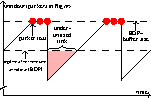
\includegraphics[width=\columnwidth]{figures/cocoa_illustration_too_little.pdf}
\caption{If the buffer is too small, loss-based \glspl{cca} cannot fully utilize the link since they send too few data following the multiplicative decrease that occurs after packet loss.}
\label{fig:tooLittle}
\end{figure}

\begin{figure}[h]
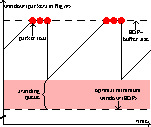
\includegraphics[width=\columnwidth]{figures/cocoa_illustration_too_much.pdf}
\caption{If the buffer is too large, loss-based \glspl{cca} keep an unnecessary standing queue not required for achieving full link utilization.}
\label{fig:tooMuch}
\end{figure}

\bibliographystyle{ACM-Reference-Format}
\bibliography{reference}

\end{document}
